

\chapter[旋转目标追踪预测]{旋转目标追踪预测}[Harbin Institute of Technology Postgraduate Dissertation Writing Specifications]

\section{引言}[Content specification]
车辆旋转会带动四周的装甲板旋转。
我们将旋转运动称之为陀螺运动。将针对于旋转目标追踪预测的算法称之为反陀螺算法。
之所以引入反陀螺算法,是因为在敌方陀螺运动下,
装甲板是圆周运动,具有强烈的非线性,而运动预测只适合线性模型。
且水平速度巨大,反复切换,出现时间短,
出现子弹还没有飞过去装甲板就已经消失的情况,需要设计专门的追踪预测算法。

\section{反陀螺模型建立}[Content specification]

基于在笛卡尔坐标系建立的全车观测模型对于观测精度的要求极高,且在中远距离以上(>4m)表现效果不佳。
于是以我方车辆为原点建立圆柱坐标系,如图ref{反陀螺坐标系}所示。原因有二:一是对于陀螺运动的敌方车辆我们更加关注于装甲板在yaw方向的运动;二是相机观测模型保证了yaw方向的观测精度。
同时,对于变量的数值我们采用相应的滤波算法处理,对于理论上不发生变换的变量我们采用均值滤波算法,对于可能发生变化的变量我们采用一阶滞后滤波算法处理。
\begin{figure}[H]
    \centering
    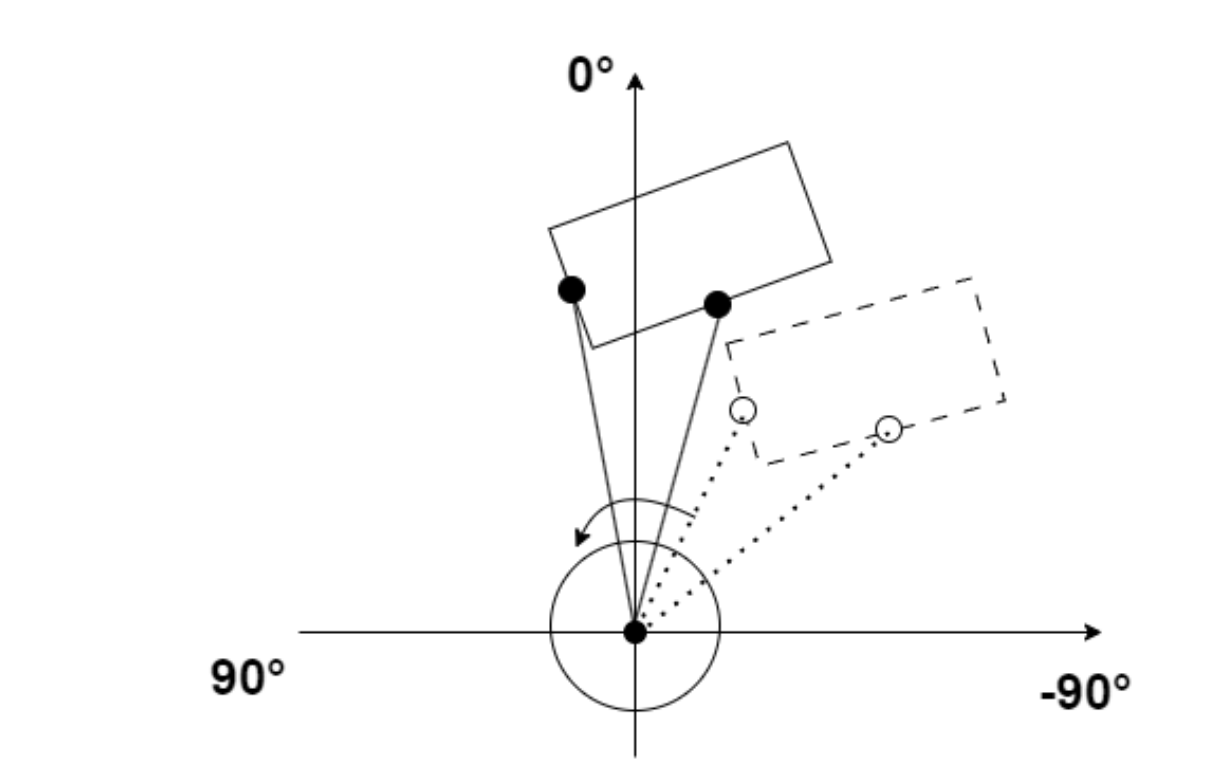
\includegraphics[width=.8\textwidth]{gyro_axis.png} 
    \caption{反陀螺坐标系} 
    \label{反陀螺坐标系}
\end{figure}



\par
在敌方车辆进行陀螺运动时,会发生装甲板切换,在装甲板切换时记录上一次的装甲板和当前装甲板,
记录为小陀螺运动的最左端和最右端。由于车辆四边都有装甲板,则在任意时刻,左右端的中间区域都会有装甲板出现,
即在任意时刻,不考虑云台响应的情况下能够命中目标。


反陀螺模型需要计算以下信息:
\begin{itemize}[itemindent=2em]
    \item 前后和左右两组装甲板的平均高度。采用均值滤波算法。
    \item 整车装甲板的平均高度。采用均值滤波算法。
    \item 陀螺周期$gyro\_period$。一次装甲板切换为0.25个周期,采用一阶滞后滤波算法处理数据,滤波系数0.2。
    \item 陀螺方向。通过角速度判断,且经过积分滤波算法处理。
    \item 最左端和最右端分别对应的$yaw\_left$和$yaw\_right$角度。采用一阶滞后滤波的形式平滑数据,滤波系数0.2。
    \item 陀螺区间$yaw\_section =0.5 \times (yaw\_left + yaw\_right)$。由于参与计算$yaw\_section$的变量已经经过滞后滤波,因此该变量不再滤波。
    \item 装甲板的平均深度信息$d$。采用一阶滞后滤波算法处理,滤波器系数0.5.
\end{itemize}

在得到这些数据后,我们就可以完全描述陀螺运动的车辆。
下图\ref{基于陀螺模型计算的yaw角度与真实yaw角度对比}展示根据陀螺模型计算的装甲板yaw角度与真实角度之差,
其中蓝色的为实时检测到目标的yaw值,红色的为利用前面的数据预测的该时刻的yaw数据。

\begin{figure}[H]
    \centering
    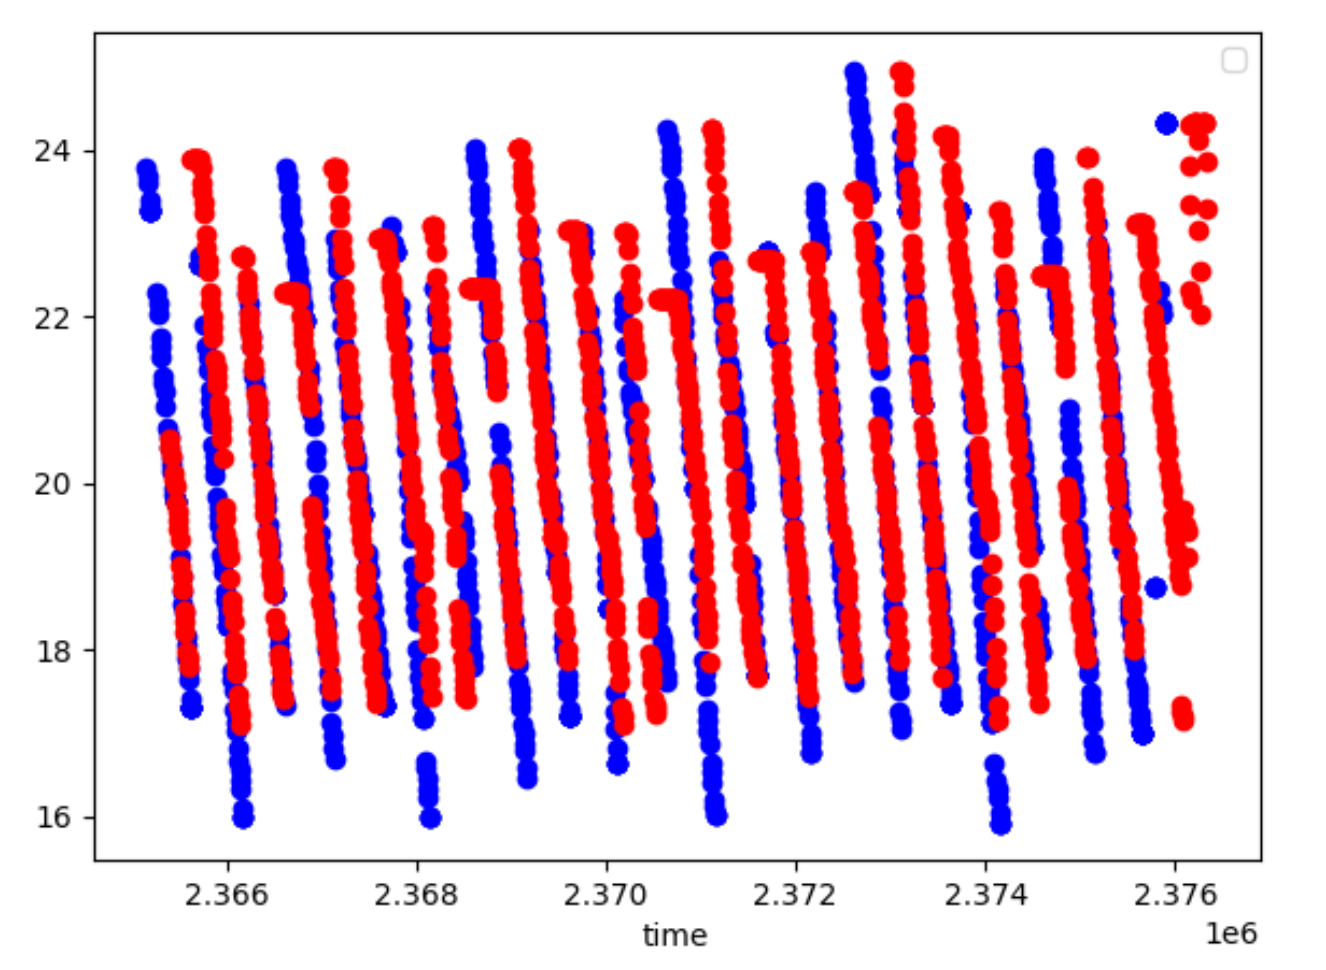
\includegraphics[width=.8\textwidth]{gyro_yaw.png} 
    \caption{反陀螺坐标系} 
    \label{基于陀螺模型计算的yaw角度与真实yaw角度对比}
\end{figure}

\section{云台姿态角求解}[Content specification]


该算法的核心是计算云台yaw和pitch姿态角。计算过程如下:
认为陀螺运动下无论是深度信息的变化(受陀螺运动和平移运动共同影响)还是装甲板高度的变换(受装甲板切换的影响,一般情况下左右和前后两组装甲板的高度不同)
对于子弹飞行时间的影响都是非常小的,即对方在陀螺运动情况下,子弹无论击打到哪个位置的装甲板飞行时间都是相同的。
因此根据上述陀螺模型计算的装甲板的平均深度信息和整车装甲板的平均高度计算子弹飞行时间,
再加入程序延时(当前时刻—上一次装甲板切换时刻),记为时间$t$。
根据时间$t$计算陀螺转了整数$n$个1/4圈,且余数为$m$。




\subsection{Pitch角度求解}[Content specification]
基于$n$计算pitch角度。
\begin{itemize}[itemindent=2em]
    \item 敌方机器人向左转,若$n$是偶数,选择右侧装甲板的高度作为弹道解算的装甲板高度。
    \item 敌方机器人向左转,若$n$是奇数,选择左侧装甲板的高度作为弹道解算的装甲板高度。
    \item 敌方机器人向右转,若$n$是偶数,选择左侧装甲板的高度作为弹道解算的装甲板高度。
    \item 敌方机器人向右转,若$n$是奇数,选择右侧装甲板的高度作为弹道解算的装甲板高度。
\end{itemize}

在得到装甲板高度信息和装甲板平均深度信息$d$后就可以求解pitch轴角度信息。

\subsection{Yaw角度求解}[Content specification]
基于$m$计算yaw角度,计算其相对于最左端或者是最右端(与转动方向有关,如果是往左传,则相对于右端,反之相对于左端)转动的yaw角度。
\begin{lstlisting}
    radio = double(4.0 * time / period)- int(4.0 * time / period);
    delta_yaw = yaw_section * radio;
\end{lstlisting}

我们将陀螺击打过程分为两个部分,云台跟随当前装甲板状态和云台回调迎接下一块装甲板状态。
云台跟随我们认为是无误差的,因为跟随量很小,但是回调量非常大,回调时间不可忽略。
考虑如下情况,对于一块从左向右(陀螺方向)旋转的装甲板,由于云台响应需要时间,
即云台并不能瞬时从最右端回调到最左端,
我们可以选择在放弃击打陀螺区间的后半程,即放弃选择击打最右端,提前将云台回调迎接下一块装甲板;也可以选择
放弃击打陀螺区间的前半程,即放弃选择击打最左端。
在分析识别算法之后发现,由于追踪算法的存在,使得检测的最右端装甲板相对于相机非常倾斜,而此时在左侧装甲板已经出现且相对于相机较为正对。
正对的装甲板不仅投影面积更大,更好击打;而且子弹与装甲板接触的法向速度更大,更不容易被裁判系统漏掉,因此选择放弃击打陀螺的后半程。
我们将选择击打的陀螺区间相对于陀螺整个区间记为r,假设云台最大角速度为$yaw\_speed_{gimbal}$,陀螺观测角速度为$yaw\_speed_{car}$
,则有如下公式:
\begin{gather}
    t  \times (yaw\_speed_{gimbal} + yaw\_speed_{car}) = yaw\_section \\
    r = \frac{t \times yaw\_speed_{gimbal} }{yaw\_section}
\end{gather}
从而求得
\begin{gather}
    r = \frac{yaw\_speed_{gimbal}}{yaw\_speed_{gimbal} + yaw\_speed_{car}}
\end{gather}

最后得到的陀螺区间角度计算公式如下(将该角度加到左端角度或右端角度)即为最终云台设定yaw角度。
\begin{lstlisting}
    radio = double(4.0 * time / period)- int(4.0 * time / period);
    r = yaw_speed_gimbal / (yaw_speed_gimbal + yaw_speed_car);
    if (radio > r) // 超出击打陀螺区间
    {
        radio = 0; // 云台提前回调
    }
    delta_yaw = yaw_section * radio;
\end{lstlisting}

\section{基于反陀螺模型求解发弹时机}[Content specification]
由于云台回调期理论上是打不中目标的,因此这一阶段我们选择不发弹。
即通过判断子弹飞过去的时间对应的装甲板所处区间,
如果区间位于radio以内,则允许发弹,否则不允许发弹。
\begin{lstlisting}
// t1 子弹飞行时间
// t2 程序时延
// t3 发弹延迟
double t = t1 + t2 + t3;
double radio_with_shoot_delay = double(4.0 * t / period) - int(4.0 * t / period);
if (radio_with_shoot_delay < radio)
{
    fire = true;
} else
{
    fire = false;
}
\end{lstlisting}



\section{基于积分滤波器的陀螺方向判断}[Content specification]

算法在每个时刻将当前的yaw\_speed累加到left\_dir\_cnt上,
从而得到一个表示yaw\_speed累积值的left\_dir\_cnt。
在每个时刻根据left\_dir\_cnt的值来判断机器人当前的旋转方向,
如果left\_dir\_cnt超过了一定阈值cnt\_thresh,
就认为机器人在相应的方向上旋转了,
并将left\_dir\_cnt重置为一个较小的值,以避免累积过多的误差。

因此,可以将该算法看作是一种积分滤波算法,
它的作用是平滑yaw\_speed信号,抑制噪声和误差的影响,从而得到更加可靠的旋转方向判断。
具体代码如下:

\begin{lstlisting}
    void AntiGyro::judge_rotate_dir(double yaw_speed, ArmorDir &dir)
    {
        const int cnt_thresh = 5;
        static int left_dir_cnt = 0;
        if (yaw_speed > 0){
            ++left_dir_cnt;
        } else if (yaw_speed < 0)
        {
            --left_dir_cnt;
        } 
        if (left_dir_cnt > cnt_thresh){
            dir = ArmorDir::LEFT;
            left_dir_cnt = 5;
        } else if (left_dir_cnt < -cnt_thresh){    
            dir = ArmorDir::RIGHT;
            left_dir_cnt = -5;
        } else {
            dir = ArmorDir::UNKNOWN;
        }
    }
\end{lstlisting}


\section{本章小结}[Content specification]

通过分析观测量的精度情况和装甲板的运动情况,在惯性系下建立反陀螺模型的圆柱坐标系,
巧妙的避开了三维坐标测量不准的情况。通过装甲板切换频率判断是否进入反陀螺模型,
基于观测的空间量和时间量计算反陀螺模式的所需信息,实现针对敌方车辆以陀螺模式运动的专门击打算法。
